\section{Technical Summary}
This API provides a comprehensive backend for a blockchain-based cryptocurrency exchange platform. It enables users to manage wallets, view transactions, authenticate, and interact with cryptocurrency data. The system is built on a modern architecture using NestJS and EdgeDB, with additional graph database capabilities through Neo4j for complex relationship queries.
\begin{table}[htbp]
\centering
\renewcommand{\arraystretch}{1.3}
\setlength{\tabcolsep}{12pt}
\begin{tabular}{|l|p{0.75\textwidth}|}
\hline
\textbf{Technology} & \textbf{Description} \\
\hline
NestJS & Progressive Node.js framework for building server-side applications \\
\hline
EdgeDB & Next-generation graph-relational database \\
\hline
Neo4j & Graph database for complex relationship queries \\
\hline
JWT & JSON Web Tokens for secure authentication \\
\hline
Swagger & API documentation and testing \\
\hline
TypeScript & Typed JavaScript for better developer experience \\
\hline
Zod & Schema validation library \\
\hline
Pino & Logging library \\
\hline
\end{tabular}
\caption{Technology Table}
\end{table}

\newpage
\section{API Architecture Diagram}
\begin{figure}[h]
    \centering
    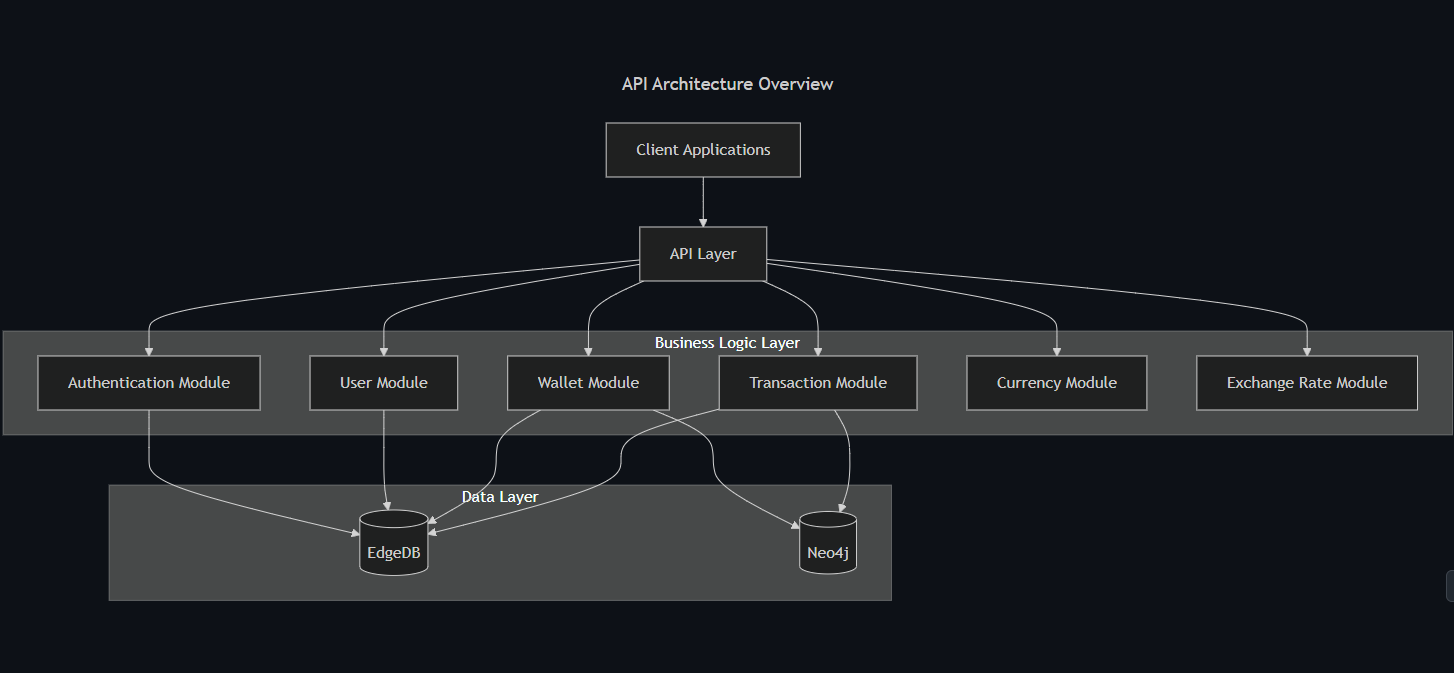
\includegraphics[width=\textwidth, keepaspectratio]{figures/api_architecture.png}
    \caption{API Architecture}
    \label{fig:api_architecture}
\end{figure}

The architecture diagram, see Figure \ref{fig:api_architecture}, illustrates a comprehensive blockchain transaction visualization system designed with a multi-layered approach:
The \textbf{Client Applications} layer serves as the user-facing interface where stakeholders interact with the blockchain data visualization tools.
The \textbf{API Layer} acts as the centralized gateway, coordinating requests and responses between client applications and the underlying business logic.
The Business Logic Layer comprises six specialized modules:
\begin{itemize}
\item \textbf{Authentication Module:} Secures access through blockchain-specific identity verification
\item \textbf{User Module:} Manages user profiles and permissions for blockchain data access
\item \textbf{Wallet Module:} Connects to and monitors blockchain wallet addresses
\item \textbf{Transaction Module:} Processes and analyzes blockchain transaction data
\item \textbf{Currency Module:} Tracks various cryptocurrencies and tokens
\item \textbf{Exchange Rate Module:} Monitors real-time cryptocurrency valuations
\end{itemize}
The Data Layer leverages two complementary database technologies:
\begin{itemize}
\item \textbf{EdgeDB:} Stores structured blockchain data, user information, and authentication details
\item \textbf{Neo4j:} Graph database optimized for blockchain transaction relationship mapping and visualization
\end{itemize}

\section{API Endpoints}

\subsection*{Authentication}
\renewcommand{\arraystretch}{1.5}
\begin{tabular}{|p{0.28\textwidth}|p{0.18\textwidth}|p{0.54\textwidth}|}
\hline
\textbf{Endpoint} & \textbf{Method} & \textbf{Description} \\
\hline
/auth/login & POST & Authenticate user and receive JWT tokens \\
\hline
/auth/refresh & GET & Refresh access token using refresh token \\
\hline
\end{tabular}

\subsection*{Users}
\renewcommand{\arraystretch}{1.5}
\begin{tabular}{|p{0.28\textwidth}|p{0.18\textwidth}|p{0.54\textwidth}|}
\hline
\textbf{Endpoint} & \textbf{Method} & \textbf{Description} \\
\hline
/users & POST & Create a new user account \\
\hline
\end{tabular}

\subsection*{Wallets}
\renewcommand{\arraystretch}{1.5}
\begin{tabular}{|p{0.38\textwidth}|p{0.12\textwidth}|p{0.5\textwidth}|}
\hline
\textbf{Endpoint} & \textbf{Method} & \textbf{Description} \\
\hline
/wallets & GET & Get all wallets with optional filtering \\
\hline
/wallets/:address & GET & Get wallet details by address \\
\hline
/wallets/:address/details & GET & Get detailed wallet information \\
\hline
/wallets/:address/transactions & GET & Get transactions for a specific wallet \\
\hline
/wallets/:address/neighbors & GET & Get wallets that have transactions with the specified wallet \\
\hline
\end{tabular}

\subsection*{Transactions}
\renewcommand{\arraystretch}{1.5}
\begin{tabular}{|p{0.38\textwidth}|p{0.12\textwidth}|p{0.5\textwidth}|}
\hline
\textbf{Endpoint} & \textbf{Method} & \textbf{Description} \\
\hline
/transactions/graph & GET & Get transaction graph data for visualization \\
\hline
\end{tabular}

\section{Request and Response Examples}
% Using boxed environment instead of black background

\subsection*{Authentication}

\subsubsection*{Login}

\textbf{Request:}

\begin{tcolorbox}[width=\textwidth, boxrule=0.5pt, colback=gray!5, colframe=gray!50]
\begin{minted}[breaklines]{bash}
POST /users
Content-Type: application/json
\end{minted}

\begin{minted}{json}
{
  "email": "user@example.com",
  "password": "securePassword123"
}
\end{minted}
\end{tcolorbox}

\vspace{1em}
\textbf{Response:}

\begin{tcolorbox}[width=\textwidth, boxrule=0.5pt, colback=gray!5, colframe=gray!50]
\begin{minted}[breaklines]{json}
{
  "accessToken": "eyJhbGciOiJIUzI1NiIsInR5cCI6IkpXVCJ9...",
  "refreshToken": "eyJhbGciOiJIUzI1NiIsInR5cCI6IkpXVCJ9..."
}
\end{minted}
\end{tcolorbox}

\subsection*{Users}

\subsubsection*{Create User}

\textbf{Request:}

\begin{tcolorbox}[width=\textwidth, boxrule=0.5pt, colback=gray!5, colframe=gray!50]
\begin{minted}[breaklines]{bash}
POST /users
Content-Type: application/json
\end{minted}

\begin{minted}[breaklines]{json}
{
  "email": "newuser@example.com",
  "password": "securePassword123",
  "firstName": "John",
  "lastName": "Doe"
}
\end{minted}
\end{tcolorbox}

\vspace{1em}
\textbf{Response:}

\begin{tcolorbox}[width=\textwidth, boxrule=0.5pt, colback=gray!5, colframe=gray!50]
\begin{minted}{json}
{
  "id": "123e4567-e89b-12d3-a456-426614174000",
  "email": "newuser@example.com",
  "firstName": "John",
  "lastName": "Doe",
  "fullName": "John Doe"
}
\end{minted}
\end{tcolorbox}

\subsection*{Wallets}

\subsubsection*{Get Wallet Details}

\textbf{Request:}

\begin{tcolorbox}[width=\textwidth, boxrule=0.5pt, colback=gray!5, colframe=gray!50]
\begin{minted}[breaklines, breakanywhere]{bash}
GET /wallets/0x742d35cc6634c0532925a3b844bc454e4438f44e/details
\end{minted}
\end{tcolorbox}

\vspace{1em}
\textbf{Response:}

\begin{tcolorbox}[width=\textwidth, boxrule=0.5pt, colback=gray!5, colframe=gray!50]
\begin{minted}{json}
{
  "address": "0x742d35cc6634c0532925a3b844bc454e4438f44e",
  "type": "EOA",
  "balance": 1.25,
  "currency": {
    "symbol": "ETH",
    "name": "Ethereum",
    "iconImg": "https://example.com/eth-icon.png"
  },
  "transactionCount": 42,
  "incomingTransactionCount": 15,
  "outgoingTransactionCount": 27
}
\end{minted}
\end{tcolorbox}

\subsection*{Get Wallet Transactions}

\textbf{Request:}

\begin{tcolorbox}[width=\textwidth, boxrule=0.5pt, colback=gray!5, colframe=gray!50]
\begin{minted}[
    breaklines=true,
    breakanywhere=true,
]{bash}
GET /wallets/0x742d35cc6634c0532925a3b844bc454e4438f44e/transactions?type=INCOMING
\end{minted}
\end{tcolorbox}


\vspace{1em}
\textbf{Response:}

\begin{tcolorbox}[width=\textwidth, boxrule=0.5pt, colback=gray!5, colframe=gray!50]
\begin{minted}[breaklines, breakanywhere=true, escapeinside=||]{json}
{
  "transactions": [
    {
      "hash": "0x1234567890abcdef1234567890abcdef1234567890abcdef",
      "value": "1000000000000000000",
      "sourceWallet": {
        "address": "0x11111222233334444555566667777888899999aaaa"
      },
      "destinationWallet": {
        "address": "0x742d35cc6634c0532925a3b844bc454e4438f44e"
      },
      "blockTimestamp": "2023-01-15T12:30:45Z",
      "transactionFee": 0.002
    }
    |\textcolor{gray}{// More transactions...}|
  ],
  "total": 15
}
\end{minted}
\end{tcolorbox}
\section{Error Handling}
The API uses standard HTTP status codes to indicate the success or failure of requests:
\begin{table}[htbp]
\centering
\renewcommand{\arraystretch}{1.3}
\setlength{\tabcolsep}{12pt}
\begin{tabular}{|l|p{0.75\textwidth}|}
\hline
\textbf{Status Code} & \textbf{Description} \\
\hline
200 & OK - The request was successful \\
\hline
201 & Created - A new resource was successfully created \\
\hline
400 & Bad Request - The request was invalid or cannot be served \\
\hline
401 & Unauthorized - Authentication is required and has failed or not been provided \\
\hline
403 & Forbidden - The server understood the request but refuses to authorize it \\
\hline
404 & Not Found - The requested resource could not be found \\
\hline
500 & Internal Server Error - An error occurred on the server \\
\hline

\end{tabular}
\caption{Status code}
\end{table}

Error responses follow this format:
\begin{tcolorbox}[width=\textwidth, boxrule=0.5pt, colback=gray!5, colframe=gray!50]
\begin{minted}[breaklines, breakanywhere=true, escapeinside=||]{json}
{
  {
  "statusCode": 400,
  "message": "Validation failed",
  "error": "Bad Request",
  "details": [
    {
      "field": "email",
      "message": "Invalid email format"
    }
  ]
}
}
\end{minted}
\end{tcolorbox}
\section{Authentication}
The API uses JWT (JSON Web Tokens) for authentication. To access protected endpoints:
\begin{enumerate}
    \item Obtain an access token by logging in via /auth/login
    \item Include the token in the Authorization header of subsequent requests:
    \begin{tcolorbox}[width=\textwidth, boxrule=0.5pt, colback=gray!5, colframe=gray!50]
\begin{minted}[
    breaklines=true,
    breakanywhere=true,
]{bash}
Authorization: Bearer <your_access_token>
\end{minted}
\end{tcolorbox}
    \item When the access token expires, use the refresh token at /auth/refresh to obtain a new access token
\begin{tcolorbox}[width=\textwidth, boxrule=0.5pt, colback=gray!5, colframe=gray!50]
\small % Adjust font size (you can also try \footnotesize or \scriptsize)
\textbf{\textcolor{red}{Warning:}} Never share your JWT tokens or store them in insecure locations.

\end{tcolorbox}
\end{enumerate}
\section{Rate Limiting}

To ensure service stability, the API implements rate limiting:
\begin{itemize}
    \item 100 requests per minute for authenticated users
    \item 20 requests per minute for unauthenticated users
\end{itemize}
\begin{tcolorbox}[width=\textwidth, boxrule=0.5pt, colback=gray!5, colframe=gray!50]
\small % Adjust font size (you can also try \footnotesize or \scriptsize)
\textbf{\textcolor{blue}{Note:}} Rate limit information is included in response headers:
\begin{itemize}
    \item \texttt{X-RateLimit-Limit}: Maximum requests allowed in the time window
    \item \texttt{X-RateLimit-Remaining}: Remaining requests in the current window
    \item \texttt{X-RateLimit-Reset}: Time when the rate limit window resets (Unix timestamp)
\end{itemize}
\end{tcolorbox}
\section{Versioning}
The API uses URL versioning. The current version is v1, which is included in the base URL:
  \begin{tcolorbox}[width=\textwidth, boxrule=0.5pt, colback=gray!5, colframe=gray!50]
\begin{minted}[
    breaklines=true,
    breakanywhere=true,
]{bash}
/api/v1/
\end{minted}
\end{tcolorbox}
\section{Getting Started}

 To start using the API:

\begin{enumerate}
  \item Register a user account via \colorbox{yellow!30}{\texttt{/users}}
  \item Authenticate via \colorbox{yellow!30}{\texttt{/auth/login}}
  \item Use the returned JWT token in the Authorization header for subsequent requests
  \item Explore wallet and transaction data using the provided endpoints
\end{enumerate}
\section{Development and Testing}
The API includes Swagger documentation accessible at  \colorbox{yellow!30}{\texttt{/api/docs}} when running in development mode.